% ============================================================
% Question Bank: ch06-02 Reproducing Scale Drawings at a Different Scale
% Topic Title: Reproducing Scale Drawings at a Different Scale
% CCSS: 7.G.A.1
% Questions: 30 (18 MC + 7 SA + 5 Graphical)
% ============================================================

% --- Multiple Choice Questions (18) ---

\begin{practiceQuestion}{6-2-q01}{mc}
\begin{questionText}
A map uses the scale $1$ cm $= 50$ km. You redraw it at $1$ cm $= 25$ km. A road that is $6$ cm on the original map becomes how long on the new map?
\end{questionText}
\choiceA{$3$ cm}
\choiceB{$6$ cm}
\choiceC{$12$ cm}
\choiceD{$150$ cm}
\correctAnswer{C}
\explanation{Scale ratio: $\frac{50}{25} = 2$. New length: $6 \times 2 = 12$ cm. The new scale is more detailed, so the drawing gets bigger.}
\end{practiceQuestion}

\begin{practiceQuestion}{6-2-q02}{mc}
\begin{questionText}
A blueprint uses $1$ cm $= 4$ m. You want to redraw it at $1$ cm $= 8$ m. A wall that is $10$ cm on the original becomes how long on the new drawing?
\end{questionText}
\choiceA{$5$ cm}
\choiceB{$10$ cm}
\choiceC{$20$ cm}
\choiceD{$40$ cm}
\correctAnswer{A}
\explanation{Scale ratio: $\frac{4}{8} = \frac{1}{2}$. New length: $10 \times \frac{1}{2} = 5$ cm. A larger scale (more real units per cm) shrinks the drawing.}
\end{practiceQuestion}

\begin{practiceQuestion}{6-2-q03}{mc}
\begin{questionText}
A model uses scale $1:100$. You need to redraw it at scale $1:50$. A wall that is $4$ cm on the original model becomes how long?
\end{questionText}
\choiceA{$2$ cm}
\choiceB{$4$ cm}
\choiceC{$8$ cm}
\choiceD{$200$ cm}
\correctAnswer{C}
\explanation{Scale ratio: $\frac{100}{50} = 2$. New length: $4 \times 2 = 8$ cm.}
\end{practiceQuestion}

\begin{practiceQuestion}{6-2-q04}{mc}
\begin{questionText}
A drawing uses $1$ cm $= 3$ m. It is redrawn at $1$ cm $= 9$ m. A room that is $12$ cm on the original becomes how long?
\end{questionText}
\choiceA{$4$ cm}
\choiceB{$12$ cm}
\choiceC{$36$ cm}
\choiceD{$108$ cm}
\correctAnswer{A}
\explanation{Scale ratio: $\frac{3}{9} = \frac{1}{3}$. New length: $12 \times \frac{1}{3} = 4$ cm.}
\end{practiceQuestion}

\begin{practiceQuestion}{6-2-q05}{mc}
\begin{questionText}
When you redraw a scale drawing at a smaller scale (more real units per cm), the new drawing is:
\end{questionText}
\choiceA{Larger than the original drawing}
\choiceB{Smaller than the original drawing}
\choiceC{The same size as the original drawing}
\choiceD{A different shape than the original drawing}
\correctAnswer{B}
\explanation{A smaller scale means each cm represents more real distance, so fewer cm are needed. The drawing gets smaller. The shape stays the same.}
\end{practiceQuestion}

\begin{practiceQuestion}{6-2-q06}{mc}
\begin{questionText}
A map uses $1$ cm $= 20$ km. You redraw it at $1$ cm $= 10$ km. What happens to the drawing?
\end{questionText}
\choiceA{Every length is halved}
\choiceB{Every length stays the same}
\choiceC{Every length is doubled}
\choiceD{Every length is multiplied by $10$}
\correctAnswer{C}
\explanation{Scale ratio: $\frac{20}{10} = 2$. Every length on the new drawing is $2$ times the old one. The drawing gets bigger because each cm now represents fewer real km.}
\end{practiceQuestion}

\begin{practiceQuestion}{6-2-q07}{mc}
\begin{questionText}
A floor plan uses $1$ cm $= 5$ ft. You redraw at $1$ cm $= 2$ ft. A room that is $3$ cm by $4$ cm on the original drawing. What is the area on the new drawing?
\end{questionText}
\choiceA{$12$ cm$^2$}
\choiceB{$30$ cm$^2$}
\choiceC{$75$ cm$^2$}
\choiceD{$150$ cm$^2$}
\correctAnswer{C}
\explanation{Scale ratio: $\frac{5}{2} = 2.5$. New dimensions: $3 \times 2.5 = 7.5$ cm and $4 \times 2.5 = 10$ cm. New area: $7.5 \times 10 = 75$ cm$^2$.}
\end{practiceQuestion}

\begin{practiceQuestion}{6-2-q08}{mc}
\begin{questionText}
A drawing uses scale $1:200$. It is redrawn at scale $1:100$. How does the area on the new drawing compare to the original?
\end{questionText}
\choiceA{It is $2$ times as large}
\choiceB{It is $4$ times as large}
\choiceC{It is half as large}
\choiceD{It is the same}
\correctAnswer{B}
\explanation{Scale ratio: $\frac{200}{100} = 2$. Lengths double, so area is multiplied by $2^2 = 4$.}
\end{practiceQuestion}

\begin{practiceQuestion}{6-2-q09}{mc}
\begin{questionText}
A map uses $1$ cm $= 40$ km. A lake is $3$ cm wide on this map. You redraw the map at $1$ cm $= 8$ km. How wide is the lake on the new map?
\end{questionText}
\choiceA{$0.6$ cm}
\choiceB{$5$ cm}
\choiceC{$15$ cm}
\choiceD{$24$ cm}
\correctAnswer{C}
\explanation{Scale ratio: $\frac{40}{8} = 5$. New width: $3 \times 5 = 15$ cm.}
\end{practiceQuestion}

\begin{practiceQuestion}{6-2-q10}{mc}
\begin{questionText}
A blueprint uses $1$ in $= 12$ ft. You redraw at $1$ in $= 4$ ft. A door that is $0.5$ in wide on the original becomes how wide?
\end{questionText}
\choiceA{$0.5$ in}
\choiceB{$1$ in}
\choiceC{$1.5$ in}
\choiceD{$3$ in}
\correctAnswer{C}
\explanation{Scale ratio: $\frac{12}{4} = 3$. New width: $0.5 \times 3 = 1.5$ in.}
\end{practiceQuestion}

\begin{practiceQuestion}{6-2-q11}{mc}
\begin{questionText}
Which of the following changes when a scale drawing is redrawn at a different scale?
\end{questionText}
\choiceA{The angles in the drawing}
\choiceB{The lengths in the drawing}
\choiceC{The shape of the figures}
\choiceD{The proportions between sides}
\correctAnswer{B}
\explanation{When you change the scale, lengths change but angles, shape, and proportions all stay the same.}
\end{practiceQuestion}

\begin{practiceQuestion}{6-2-q12}{mc}
\begin{questionText}
A map uses $1$ cm $= 30$ km. A second map uses $1$ cm $= 15$ km. A river is $4.5$ cm long on the first map. How long is it on the second map?
\end{questionText}
\choiceA{$2.25$ cm}
\choiceB{$9$ cm}
\choiceC{$15$ cm}
\choiceD{$67.5$ cm}
\correctAnswer{B}
\explanation{Scale ratio: $\frac{30}{15} = 2$. New length: $4.5 \times 2 = 9$ cm.}
\end{practiceQuestion}

\begin{practiceQuestion}{6-2-q13}{mc}
\begin{questionText}
A drawing uses $1$ cm $= 6$ m. It is redrawn at $1$ cm $= 2$ m. The original drawing is $8$ cm by $5$ cm. What is the perimeter of the new drawing?
\end{questionText}
\choiceA{$26$ cm}
\choiceB{$39$ cm}
\choiceC{$78$ cm}
\choiceD{$120$ cm}
\correctAnswer{C}
\explanation{Scale ratio: $\frac{6}{2} = 3$. New dimensions: $8 \times 3 = 24$ cm and $5 \times 3 = 15$ cm. New perimeter: $2(24 + 15) = 78$ cm.}
\end{practiceQuestion}

\begin{practiceQuestion}{6-2-q14}{mc}
\begin{questionText}
Original scale: $1$ cm $= 10$ m. New scale: $1$ cm $= 40$ m. What is the scale ratio?
\end{questionText}
\choiceA{$\frac{1}{4}$}
\choiceB{$4$}
\choiceC{$30$}
\choiceD{$\frac{1}{30}$}
\correctAnswer{A}
\explanation{Scale ratio: $\frac{10}{40} = \frac{1}{4}$. Every old length is multiplied by $\frac{1}{4}$ on the new drawing.}
\end{practiceQuestion}

\begin{practiceQuestion}{6-2-q15}{mc}
\begin{questionText}
A floor plan uses $1$ cm $= 3$ ft. A room is $6$ cm long on this plan. If the same room is $2$ cm long on a new plan, what scale does the new plan use?
\end{questionText}
\choiceA{$1$ cm $= 1$ ft}
\choiceB{$1$ cm $= 6$ ft}
\choiceC{$1$ cm $= 9$ ft}
\choiceD{$1$ cm $= 12$ ft}
\correctAnswer{C}
\explanation{Actual length: $6 \times 3 = 18$ ft. On the new plan: $18 \div 2 = 9$ ft per cm. New scale: $1$ cm $= 9$ ft.}
\end{practiceQuestion}

\begin{practiceQuestion}{6-2-q16}{mc}
\begin{questionText}
A model uses scale $1:25$. A new model uses scale $1:75$. A window that is $6$ cm on the first model becomes how long on the second?
\end{questionText}
\choiceA{$2$ cm}
\choiceB{$6$ cm}
\choiceC{$18$ cm}
\choiceD{$150$ cm}
\correctAnswer{A}
\explanation{Scale ratio: $\frac{25}{75} = \frac{1}{3}$. New length: $6 \times \frac{1}{3} = 2$ cm.}
\end{practiceQuestion}

\begin{practiceQuestion}{6-2-q17}{mc}
\begin{questionText}
A map uses $1$ cm $= 60$ km. You redraw it at $1$ cm $= 20$ km. A triangle on the original has an area of $4$ cm$^2$. What is its area on the new map?
\end{questionText}
\choiceA{$12$ cm$^2$}
\choiceB{$16$ cm$^2$}
\choiceC{$36$ cm$^2$}
\choiceD{$48$ cm$^2$}
\correctAnswer{C}
\explanation{Scale ratio: $\frac{60}{20} = 3$. Area scales by $3^2 = 9$. New area: $4 \times 9 = 36$ cm$^2$.}
\end{practiceQuestion}

\begin{practiceQuestion}{6-2-q18}{mc}
\begin{questionText}
A drawing uses $1$ cm $= 5$ km. A road is $7$ cm long. Another map shows the same road as $3.5$ cm. What is the scale of the second map?
\end{questionText}
\choiceA{$1$ cm $= 2.5$ km}
\choiceB{$1$ cm $= 5$ km}
\choiceC{$1$ cm $= 10$ km}
\choiceD{$1$ cm $= 17.5$ km}
\correctAnswer{C}
\explanation{Actual road: $7 \times 5 = 35$ km. New scale: $35 \div 3.5 = 10$. So the second map uses $1$ cm $= 10$ km.}
\end{practiceQuestion}

% --- Short Answer Questions (7) ---

\begin{practiceQuestion}{6-2-q19}{sa}
\begin{questionText}
A drawing uses $1$ cm $= 12$ m. You redraw at $1$ cm $= 4$ m. A hallway is $5$ cm on the original. How long is it on the new drawing?
\end{questionText}
\correctAnswer{$15$ cm}
\explanation{Scale ratio: $\frac{12}{4} = 3$. New length: $5 \times 3 = 15$ cm.}
\end{practiceQuestion}

\begin{practiceQuestion}{6-2-q20}{sa}
\begin{questionText}
A map uses $1$ cm $= 100$ km. You redraw at $1$ cm $= 25$ km. A distance is $3$ cm on the original. How long is it on the new map?
\end{questionText}
\correctAnswer{$12$ cm}
\explanation{Scale ratio: $\frac{100}{25} = 4$. New length: $3 \times 4 = 12$ cm.}
\end{practiceQuestion}

\begin{practiceQuestion}{6-2-q21}{sa}
\begin{questionText}
A blueprint uses scale $1:80$. You redraw at scale $1:20$. A room is $2$ cm by $3$ cm on the original. What is the area of the room on the new drawing?
\end{questionText}
\correctAnswer{$96$ cm$^2$}
\explanation{Scale ratio: $\frac{80}{20} = 4$. New dimensions: $2 \times 4 = 8$ cm and $3 \times 4 = 12$ cm. New area: $8 \times 12 = 96$ cm$^2$.}
\end{practiceQuestion}

\begin{practiceQuestion}{6-2-q22}{sa}
\begin{questionText}
A floor plan uses $1$ cm $= 6$ ft. On this plan, a room is $9$ cm long. On a second plan, the same room is $3$ cm long. What scale does the second plan use?
\end{questionText}
\correctAnswer{$1$ cm $= 18$ ft}
\explanation{Actual length: $9 \times 6 = 54$ ft. New scale: $54 \div 3 = 18$ ft per cm.}
\end{practiceQuestion}

\begin{practiceQuestion}{6-2-q23}{sa}
\begin{questionText}
A park is drawn at scale $1$ cm $= 50$ m. The park is $8$ cm wide on this drawing. If the new drawing must show the park as $4$ cm wide, what scale should the new drawing use?
\end{questionText}
\correctAnswer{$1$ cm $= 100$ m}
\explanation{Actual width: $8 \times 50 = 400$ m. New scale: $400 \div 4 = 100$ m per cm.}
\end{practiceQuestion}

\begin{practiceQuestion}{6-2-q24}{sa}
\begin{questionText}
A drawing uses $1$ cm $= 7$ m. You redraw at $1$ cm $= 7$ m (the same scale). A line is $5$ cm long. How long is it on the new drawing?
\end{questionText}
\correctAnswer{$5$ cm}
\explanation{The scale ratio is $\frac{7}{7} = 1$. The length stays the same: $5 \times 1 = 5$ cm.}
\end{practiceQuestion}

\begin{practiceQuestion}{6-2-q25}{sa}
\begin{questionText}
A map uses $1$ cm $= 15$ km. A trail is $8$ cm on this map. On a new map, the trail is $24$ cm. What is the scale ratio from old to new?
\end{questionText}
\correctAnswer{$3$}
\explanation{$24 \div 8 = 3$. Every old measurement is multiplied by $3$ on the new map.}
\end{practiceQuestion}

% --- Graphical Questions (3 GMC + 2 GSA) ---

\begin{practiceQuestion}{6-2-q26}{gmc}
\begin{questionText}
The original drawing below uses scale $1$ cm $= 10$ m. You are asked to redraw the rectangle at scale $1$ cm $= 5$ m. What will the new dimensions be?

\begin{center}
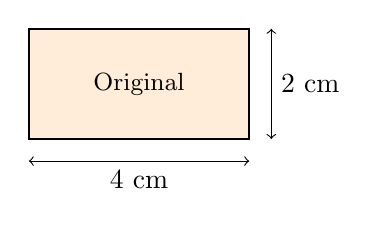
\begin{tikzpicture}[scale=0.7]
  \draw[thick,fill=orange!15] (0,0) rectangle (4,2);
  \draw[<->] (0,-0.4) -- (4,-0.4);
  \node[below] at (2,-0.4) {$4$ cm};
  \draw[<->] (4.4,0) -- (4.4,2);
  \node[right] at (4.4,1) {$2$ cm};
  \node at (2,1) {\small Original};
\end{tikzpicture}
\end{center}
\end{questionText}
\choiceA{$2$ cm by $1$ cm}
\choiceB{$4$ cm by $2$ cm}
\choiceC{$8$ cm by $4$ cm}
\choiceD{$20$ cm by $10$ cm}
\correctAnswer{C}
\explanation{Scale ratio: $\frac{10}{5} = 2$. New dimensions: $4 \times 2 = 8$ cm by $2 \times 2 = 4$ cm.}
\end{practiceQuestion}

\begin{practiceQuestion}{6-2-q27}{gmc}
\begin{questionText}
The two rectangles below represent the same room drawn at two different scales. The original uses $1$ cm $= 6$ m. What scale does the new drawing use?

\begin{center}
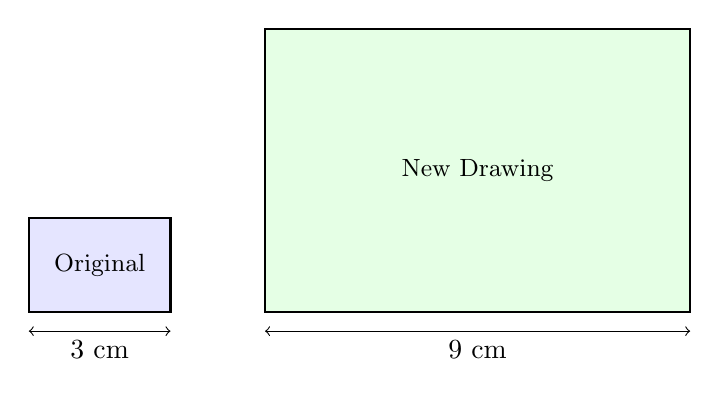
\begin{tikzpicture}[scale=0.6]
  % Original
  \draw[thick,fill=blue!10] (0,0) rectangle (3,2);
  \node at (1.5,1) {\small Original};
  \draw[<->] (0,-0.4) -- (3,-0.4);
  \node[below] at (1.5,-0.4) {$3$ cm};
  % New
  \draw[thick,fill=green!10] (5,0) rectangle (14,6);
  \node at (9.5,3) {\small New Drawing};
  \draw[<->] (5,-0.4) -- (14,-0.4);
  \node[below] at (9.5,-0.4) {$9$ cm};
\end{tikzpicture}
\end{center}
\end{questionText}
\choiceA{$1$ cm $= 2$ m}
\choiceB{$1$ cm $= 3$ m}
\choiceC{$1$ cm $= 6$ m}
\choiceD{$1$ cm $= 18$ m}
\correctAnswer{A}
\explanation{Scale ratio: $9 \div 3 = 3$. The new drawing is $3$ times bigger. Actual length: $3 \times 6 = 18$ m. New scale: $18 \div 9 = 2$ m per cm.}
\end{practiceQuestion}

\begin{practiceQuestion}{6-2-q28}{gmc}
\begin{questionText}
A triangle on Drawing A (scale $1$ cm $= 4$ m) has the dimensions shown below. Drawing B uses scale $1$ cm $= 2$ m. What is the base of the triangle on Drawing B?

\begin{center}
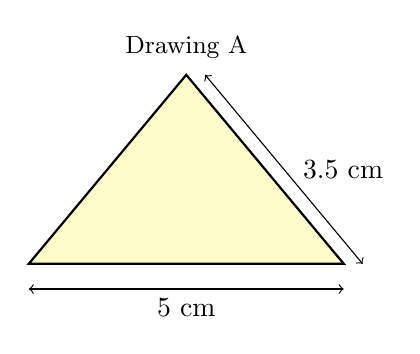
\begin{tikzpicture}[scale=0.8]
  \draw[thick,fill=yellow!20] (0,0) -- (5,0) -- (2.5,3) -- cycle;
  \draw[<->] (0,-0.4) -- (5,-0.4);
  \node[below] at (2.5,-0.4) {$5$ cm};
  \draw[<->] (5.3,0) -- (2.8,3);
  \node[right] at (4.2,1.5) {$3.5$ cm};
  \node[above] at (2.5,3.1) {\small Drawing A};
\end{tikzpicture}
\end{center}
\end{questionText}
\choiceA{$2.5$ cm}
\choiceB{$5$ cm}
\choiceC{$10$ cm}
\choiceD{$20$ cm}
\correctAnswer{C}
\explanation{Scale ratio: $\frac{4}{2} = 2$. New base: $5 \times 2 = 10$ cm.}
\end{practiceQuestion}

\begin{practiceQuestion}{6-2-q29}{gsa}
\begin{questionText}
The rectangle below is drawn at scale $1$ cm $= 8$ m. Redraw it at scale $1$ cm $= 4$ m. What are the new dimensions, and what is the new drawing's area?

\begin{center}
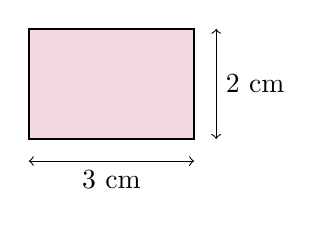
\begin{tikzpicture}[scale=0.7]
  \draw[thick,fill=purple!15] (0,0) rectangle (3,2);
  \draw[<->] (0,-0.4) -- (3,-0.4);
  \node[below] at (1.5,-0.4) {$3$ cm};
  \draw[<->] (3.4,0) -- (3.4,2);
  \node[right] at (3.4,1) {$2$ cm};
\end{tikzpicture}
\end{center}
\end{questionText}
\correctAnswer{$6$ cm by $4$ cm; area $= 24$ cm$^2$}
\explanation{Scale ratio: $\frac{8}{4} = 2$. New dimensions: $3 \times 2 = 6$ cm and $2 \times 2 = 4$ cm. Area: $6 \times 4 = 24$ cm$^2$.}
\end{practiceQuestion}

\begin{practiceQuestion}{6-2-q30}{gsa}
\begin{questionText}
The grid below shows a house floor plan at scale $1$ square $= 3$ m. The shaded region represents the kitchen. If you redraw the plan at $1$ square $= 1$ m, how many grid squares will the new kitchen cover?

\begin{center}
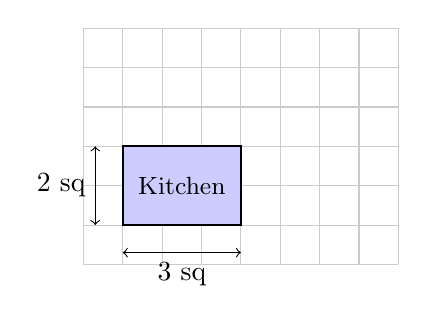
\begin{tikzpicture}[scale=0.5]
  \draw[step=1,gray!40,thin] (0,0) grid (8,6);
  \fill[blue!20] (1,1) rectangle (4,3);
  \draw[thick] (1,1) rectangle (4,3);
  \node at (2.5,2) {\small Kitchen};
  \draw[<->] (1,0.3) -- (4,0.3);
  \node[below] at (2.5,0.3) {$3$ sq};
  \draw[<->] (0.3,1) -- (0.3,3);
  \node[left] at (0.3,2) {$2$ sq};
\end{tikzpicture}
\end{center}
\end{questionText}
\correctAnswer{$54$ grid squares}
\explanation{Original kitchen: $3$ squares by $2$ squares $= 6$ squares. Each original square represents $3$ m, new square represents $1$ m. Scale ratio for length: $\frac{3}{1} = 3$. New dimensions: $3 \times 3 = 9$ squares by $2 \times 3 = 6$ squares. New area: $9 \times 6 = 54$ grid squares.}
\end{practiceQuestion}
